% !BIB TS-program = biber
\documentclass[final, journal, 11pt]{report}
\usepackage[utf8]{inputenc}
\usepackage[margin=8em]{geometry}
\usepackage{graphicx}
\usepackage{amsmath}
\usepackage{amsthm}
\usepackage{enumitem}
\usepackage{booktabs}
\usepackage{makecell}
\usepackage{tikz}
\usepackage{authblk}
\usepackage{amssymb}
\usepackage{biblatex}
\usepackage{listings}
\usepackage{capt-of}
\usepackage{booktabs}
\usepackage{lipsum}
\usepackage{hyperref}

\lstset{
	language=Python,
	basicstyle=\ttfamily\small,                 % Use a small monospaced font
	keywordstyle=\color{blue},                   % Keywords in blue
	stringstyle=\color{brown},                   % Strings in brown
	commentstyle=\color{green!60!black},         % Comments in dark green
	backgroundcolor=\color{white},               % White background
	frame=single,                               % Add a frame around the code
	breaklines=true,                             % Break long lines
	numbers=left,                               % Add line numbers on the left
	numberstyle=\tiny\color{gray},               % Line numbers in gray
	stepnumber=1,                               % Number every line
	numbersep=5pt,                              % Distance from line numbers to code
	showstringspaces=false,                      % Don't show spaces in strings
	emphstyle=\color{purple},                    % Style for emphasized words
	tabsize=4                                    % Set tab size to 4 spaces
}


\usetikzlibrary{shapes, arrows, shadings, positioning}

\addbibresource{refs.bib}

\setlength{\parindent}{0em}
\setlength{\parskip}{1em}

\usepackage{url}
\title{\textbf{Maze solving using Intelligent Agents}}
\author{Aman~Pathak$^{1}$}

\affil{$^1$Kalinga Institute of Industrial Technology, Bhubaneshwar\\{\footnotesize apathakcse@gmail.com}}
\date{}

\begin{document}
	\maketitle
	
	\section*{Abstract}
	This report presents a mini-project on AI-powered maze solving using intelligent agents. The codebase implements both unidirectional and bidirectional versions of Breadth-First Search (BFS) and Depth-First Search (DFS). A comprehensive analysis of algorithms in terms of time complexity, space complexity, and path optimality is conducted. Performance is compared using metrics such as the number of nodes explored, execution time, and memory usage.
	
	\section*{Introduction}
	
	A maze-solving algorithm systematically identifies a path through a maze. These algorithms are categorized based on the solver's perspective:
	
	\begin{enumerate}
	\item "Inside the maze" algorithms - Examples include random mouse, wall follower, Pledge, and Trémaux's methods. These are suitable for scenarios where the solver can only observe their immediate environment, akin to navigating a maze physically.

	\item "Full view" algorithms - Examples include dead-end filling and shortest path methods. These are applicable when the entire maze layout is visible, as in the case of a computer program analyzing the complete maze structure.
	\end{enumerate}

	
	In the case of a maze without loops, known as a "perfect" or "simply connected" maze, it is mathematically equivalent to a tree in graph theory. This can be visualized by extending all maze paths to create a branching tree structure. This relationship with graph theory underlies the foundation of many maze-solving techniques based on graph algorithms.
	
	Maze solving is a classic problem in artificial intelligence, requiring an agent to find a route from a starting point to a goal within a defined environment. This project implements BFS and DFS algorithms in their unidirectional and bidirectional forms to evaluate their performance and suitability for this task. The focus lies on comparing their efficiency, memory requirements, and the optimality of solutions.
	
	
	\section*{Problem Description}
	The maze is represented as a graph where nodes correspond to positions within the maze, and edges represent possible movements between positions. The problem is to determine a sequence of movements from the start node to the goal node. The solution should minimize computational resources while ensuring correctness.
	
	\section*{Algorithms Implemented}
	
	\subsection*{Maze Generator}
	
	We implemented the \texttt{generate\_maze} algorithm to generate a randomized maze with a specified size and open path density. The maze is represented as a two-dimensional grid, where walls are denoted by \# and open paths are denoted by \texttt{.}. The algorithm accepts three input parameters: \texttt{length} (the number of rows), \texttt{breadth} (the number of columns), and \texttt{path\_usage\_percentage}, which defines the percentage of the maze that will consist of open paths. 
	
	The algorithm begins by creating a maze of dimensions \texttt{length} x \texttt{breadth}, initially filled with walls (\#). We then randomly choose coordinates for the start point, denoted \texttt{S}, and the end point, denoted \texttt{E}. If the start and end points coincide, we repeat the process until they are distinct. The start and end points are then placed in the maze.
	
	Next, we calculate the number of open cells based on the \texttt{path\_usage\_percentage}, which controls how much of the maze is open. Starting from the initial set of visited cells, which includes the start point, we randomly select additional cells and mark them as open (\texttt{.}) until the desired number of open cells is reached. The start and end points remain unchanged, ensuring they are always part of the maze.
	
	Finally, we return the maze as a two-dimensional list, where each cell is either a wall (\#), an open path (\texttt{.}), or one of the special points (\texttt{S} for start and \texttt{E} for end). The resulting maze may not necessarily be fully connected, meaning there is no guarantee that a path exists between \texttt{S} and \texttt{E}, but the density of open paths is controlled by the \texttt{path\_usage\_percentage} parameter.
	
	This ensures that we generate unbiased random mazes on every run.
	
	
	\subsection*{Breadth-First Search (BFS)}
	
	Breadth-first search (BFS) is a systematic approach to exploring a problem space where the goal is to find the shortest path between two nodes or states. It works by examining all possible moves or paths within a given "radius" before expanding outward. This ensures that once a valid path is found, it is guaranteed to be the shortest. For instance, in an infinite or large array of cells, BFS explores all nearby cells first, progressively moving outward until the target is reached. This radius-based exploration prevents the algorithm from wandering off in the wrong direction indefinitely, making BFS particularly effective in scenarios where the shortest path is critical.
	

	
	\begin{lstlisting}
def find_path_bfs(maze):
    """
    Find the path from 'S' to 'E' using Breadth-First Search and return all states.

    Args:
        maze (list): The maze represented as a 2D list.

    Returns:
        tuple: (final_maze, maze_states) where final_maze is the solved maze and 
               maze_states is a list of all intermediate states. Returns (None, [])
               if no path exists.
    """
	\end{lstlisting}
	
		\begin{figure}[!htbp]
			\centering
			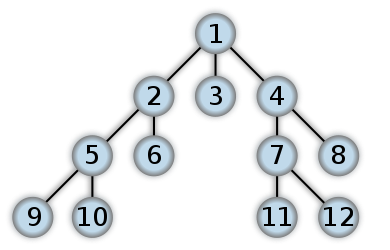
\includegraphics[width=2.6in]{assets/BFS.png}
			\caption{A tree labeled by the order in which BFS expands its nodes}
			\label{fig:BFS}
		\end{figure} 
		
	
	
	\subsection*{Depth-First Search (DFS)}
	DFS explores as far as possible along each branch before backtracking. It uses a stack and does not guarantee optimal solutions. It dives deep into a single path of the problem space before backtracking when necessary. This approach requires less memory because it only needs to maintain the current state and apply or undo moves as it progresses. DFS is highly efficient in finite problem spaces with high branching factors, as it avoids the need to keep track of all possible states simultaneously. However, in infinite or very large spaces, DFS can become inefficient if it pursues incorrect paths for extended periods. Its strength lies in its simplicity and memory efficiency in contained, well-defined search spaces.
	

	
	\begin{lstlisting}
def find_path_dfs(maze):
    """
    Find the path from 'S' to 'E' using Depth-First Search and return all states.

    Args:
        maze (list): The maze represented as a 2D list.

    Returns:
        tuple: (final_maze, maze_states) where final_maze is the solved maze and 
               maze_states is a list of all intermediate states. Returns (None, [])
               if no path exists.
    """
	\end{lstlisting}
	
	\begin{figure}[!htbp]
		\centering
		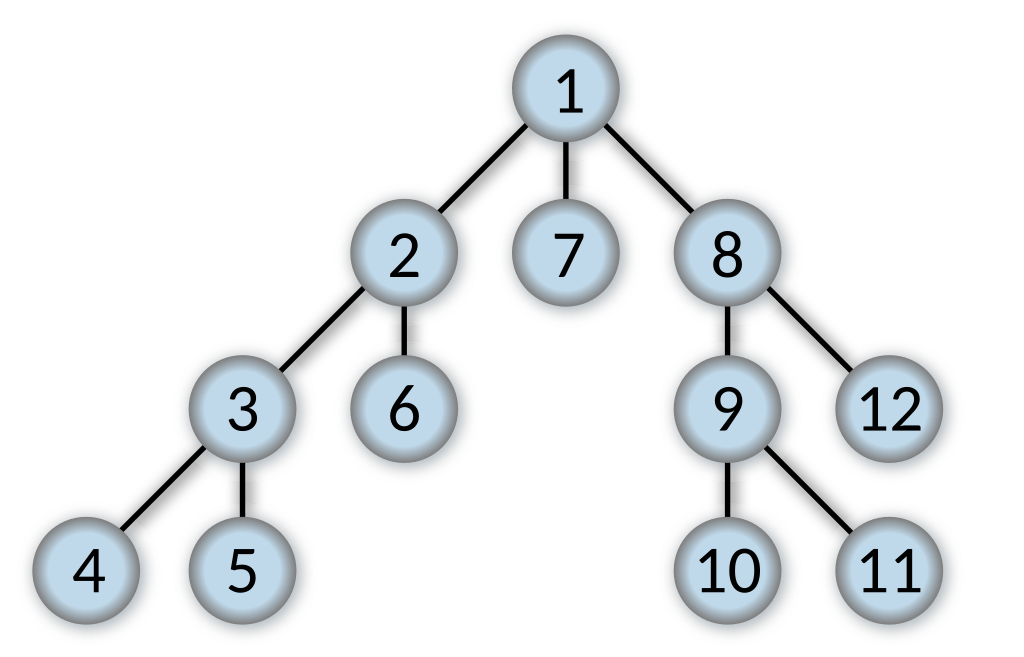
\includegraphics[width=2.6in]{assets/DFS.png}
		\caption{A tree labeled by the order in which DFS expands its nodes}
		\label{fig:DFS}
	\end{figure} 
	
	\subsection*{Bidirectional Search}
	Bidirectional search is a flexible strategy that can utilize either breadth-first search (BFS) or depth-first search (DFS), based on the specific requirements of the problem. The main concept involves launching searches from both the start node and the goal node simultaneously, with the objective of meeting in the middle. This method effectively minimizes the search space by dividing the problem into two smaller subproblems, each requiring less depth to explore. Regardless of whether BFS or DFS is employed, the key benefit is the reduction of the exponential growth of states that would need exploration in a unidirectional search. BFS guarantees the shortest path when applied bidirectionally, while DFS may be preferred in situations where memory efficiency or rapid exploration of deeper paths is essential. The adaptability of bidirectional search makes it a valuable technique for efficiently addressing large, finite search problems.
	
	\section*{Time Complexity}
	
	\subsection*{Unidirectional}
	The time complexity of both the \texttt{find\_path\_bfs} and \texttt{find\_path\_dfs} functions is dominated by the traversal over the maze. In the worst case, both algorithms visit each cell in the maze at most once. The maze consists of \( R \) rows and \( C \) columns, so the total number of cells is \( R \times C \).
	
	In the case of \texttt{find\_path\_bfs}, the algorithm uses a queue to manage the cells to visit. For each cell, it checks its four neighbors (up, down, left, and right), which results in \( O(1) \) operations per cell. Since the BFS traversal processes all \( R \times C \) cells, the overall time complexity for the BFS traversal is \( O(R \times C) \).
	
	Similarly, in \texttt{find\_path\_dfs}, the algorithm uses a stack to manage the cells to visit. It also checks the four neighbors of each cell, resulting in \( O(1) \) operations per cell. Like BFS, the DFS traversal processes all \( R \times C \) cells, so its time complexity is also \( O(R \times C) \).
	
	In both algorithms, for each visited cell, a copy of the maze is generated to store the intermediate state. Since copying the maze takes \( O(R \times C) \) time and a copy is made for each visited cell, this adds another \( O(R \times C) \) factor for state creation.
	
	Therefore, the overall time complexity for both the BFS and DFS functions is \( O(R \times C) \), as both algorithms perform equivalent operations in terms of visiting cells and generating maze states.
	
	\subsection*{Bidirectional}
	The time complexity of the \texttt{find\_path\_bfs\_bidirectional} function is similar to that of regular BFS, with no improvement in the upper bound of the time complexity. In the worst case, both the forward search (from 'S') and the backward search (from 'E') will visit a subset of the maze cells. Since the maze has \( R \) rows and \( C \) columns, there are \( R \times C \) cells in total. Each search explores roughly half of the maze, so the total number of cells visited by both searches is \( O(R \times C) \).
	
	The bidirectional BFS expands from both the start and the end simultaneously. Each side performs a constant amount of work for each visited cell, specifically \( O(1) \) operations. Although the effective number of visited cells is reduced by half, the upper bound of the time complexity remains \( O(R \times C) \).
	
	In practice, the running time is likely to improve because the two searches meet sooner, reducing the number of operations compared to a single-sided BFS. In ideal conditions, the running time could be approximately halved, as the search space is divided into two smaller parts. However, this reduction is not guaranteed in all cases, and the worst-case complexity remains \( O(R \times C) \).
	
	Similarly, the time complexity of the \texttt{find\_path\_dfs\_bidirectional} function mirrors that of bidirectional BFS. In the worst case, both the forward and backward searches will visit a subset of the maze cells, so the total number of cells visited is \( O(R \times C) \). Each search performs \( O(1) \) operations for each visited cell. 
	
	Bidirectional DFS expands from both the start and end simultaneously, and while the effective number of visited cells is reduced, the upper bound of the time complexity remains \( O(R \times C) \).
	
	
	
	
	
	
	
	
	
	
	\subsection*{Space Complexity}
		Both Breadth-First Search (BFS) and Depth-First Search (DFS) have equivalent upper tight bounds for space complexity, despite their different traversal strategies. In the case of BFS, the queue stores tuples of coordinates along with the path, and in the worst case, it can store all positions in the maze, leading to a space complexity of \( O(R \times C) \), where \( R \) and \( C \) are the number of rows and columns in the maze. Similarly, DFS uses a stack to store coordinates and paths, and it can also store all positions in the maze in the worst case, resulting in the same space complexity of \( O(R \times C) \). In both algorithms, the visited set also stores all coordinates that have been visited, contributing another \( O(R \times C) \) space. Additionally, the \texttt{maze\_states} list, which stores copies of the maze at each step, contributes \( O(R^2 C^2) \) space in both cases. In general, the algorithm itself has a space complexity of \( O(R \times C) \); however, due to our specific implementation and the requirement for visualizing each step, there exists an overhead in space complexity, which results in an upper bound of \( O(R^2 C^2) \). Thus, while BFS and DFS differ in their traversal order, their overall space complexity, dominated by the storage of intermediate maze states, is equivalent, with an upper bound of \( O(R^2 C^2) \).
		
		The effective space complexity of Bidirectional Breadth-First Search (BFS) and Bidirectional Depth-First Search (DFS) is identical to that of their unidirectional counterparts, BFS and DFS, despite the bidirectional approach aiming to speed up the search by exploring from both the start and end simultaneously. This is because, in the worst case, both directions will explore all nodes independently, just as in the unidirectional case. Bidirectional BFS and DFS do use two queues or stacks (one for each direction) and two sets for tracking visited nodes, but this does not increase the overall space complexity. Each direction still only requires \(O(R \times C)\) space for the visited nodes, and thus the combined space complexity for both directions remains proportional to \(O(R \times C)\), which is the same as that of unidirectional BFS and DFS. The extra space needed for storing intermediate maze states during exploration does contribute to the overall space complexity, but the primary space complexity is still determined by the visited nodes and auxiliary structures. Hence, the effective space complexity for bidirectional searches is still \(O(R \times C)\), just like unidirectional searches.
		
		
		
	
	
	\section*{Path Optimality}
		\subsection*{BFS}
		
		Breadth-First Search (BFS) is optimal when the path cost is a nondecreasing function of the depth of the node. The most common such scenario is when all actions have the same cost. As stated by Russell and Norvig,
		
		\begin{quote}
		    "Breadth-First Search is optimal if the path cost is a nondecreasing function of the depth of the node."
		\end{quote}
		
		In the context of maze solving, the cost of moving in any direction (up, down, left, or right) is constant. Since all actions have the same cost, BFS is optimal for finding the shortest path in a maze, as it explores all possible paths level by level and guarantees that the first time it reaches the goal, it has found the shortest possible path.
		
		\subsection*{DFS}
		Depth-First Search (DFS) is not guaranteed to find the optimal solution because it does not prioritize exploring the shortest path first. This means that the first solution found by DFS is not necessarily the best or optimal one, as DFS might explore longer paths before reaching the goal. In contrast, Breadth-First Search (BFS), while not optimal in all cases, ensures that the shortest path is found if all actions have the same cost. However, neither DFS nor BFS is optimal in a general sense, as they do not account for differing action costs or path lengths. In AI, the optimal strategy refers to the one that maximizes utility or guarantees the best result, but in many cases, especially in complex problems, the specific case is unknown, and we can only hypothesize which strategy will work best. DFS can, however, be considered optimal in specific scenarios, such as when the search tree is finite, all action costs are identical, and all solutions are of the same length. This is the case for Constraint Satisfaction Problems (CSPs), where DFS can efficiently find the optimal solution under these constraints. It is important to note that DFS is optimal under these conditions only when certain bounds are applied, such as limiting the depth of the search tree or restricting the length of solutions. In the absence of such bounds, DFS is not considered optimal, especially when compared to algorithms like A*, which are designed to handle weighted actions and return the shortest path.
		
		\subsection*{Bidrectional BFS}
		Bidirectional Breadth-First Search (BBFS) is optimal in the sense that it finds the shortest path between the start and end nodes. This is because:
		
		\textbf{Completeness:} BBFS is complete, meaning it will find a path if one exists, provided that the graph is connected and both the start and end nodes are reachable from each other. 
		
		\textbf{Optimality:} The algorithm terminates when the two BFSs meet, ensuring that the path found is the shortest possible. Each BFS explores the graph level by level, starting from the start and end nodes. The intersection of the two BFSs occurs at the node with the minimum distance from both directions, guaranteeing that the path found is the shortest, as both searches expand equally towards each other. This results in finding the optimal path in terms of the number of steps, making BBFS an optimal algorithm for finding the shortest path in an unweighted graph.
		
		\subsection*{Bidirectional DFS}
		Bidirectional Depth-First Search (BDDFS) is optimal in the sense that it can find the shortest path between the start and end nodes under specific conditions. This is because:
		
		\textbf{Completeness:} BDDFS is complete as long as the search space is finite and both the start and end nodes are reachable. The algorithm explores from both directions (start and end) simultaneously, and the search continues until the two searches meet, ensuring that the search does not miss a path if one exists.
		
		\textbf{Optimality:} While BDDFS is not guaranteed to always find the shortest path in all cases, it is optimal when applied under certain conditions. Specifically, BDDFS can find the optimal solution if the search space is finite, all action costs are identical, and all solutions have the same length. This is because both searches expand evenly from the start and end, and when they meet, they form the shortest path between the two points. However, BDDFS may not be optimal in graphs with varying action costs or when solutions have different lengths, as it does not prioritize the shortest path as BFS does.
		
		
	
	\section*{Performance Comparison}
	Performance metrics are evaluated across the following dimensions:
	\begin{itemize}
		\item \textbf{Nodes Explored:} BFS typically explores fewer nodes than DFS due to its systematic approach.
		\item \textbf{Execution Time:} BFS and DFS have comparable time complexity, where bidirectional search often reduces runtime.
		\item \textbf{Memory Usage:} DFS generally requires less memory than BFS.
	\end{itemize}
	
	The latest codebase for this project can be found at \href{https://github.com/vajradevam/ai-lab}{https://github.com/vajradevam/ai-lab}.
	
	\begin{table}[!htbp]
	\centering
	\begin{tabular}{@{}ccccccc@{}}
	\toprule
	\textbf{Slno} & \textbf{Algo} & \textbf{Visited} & \textbf{Shortest Path} & \textbf{Time} & \textbf{Current Mem} & \textbf{Peak Mem} \\ \midrule
	1 & BFS       & 672  & 25   & 0.05 s & 10.94 MB & 19.60 MB \\
	  & DFS       & 613  & 314  & 0.05 s & 9.48 MB  & 9.86 MB  \\
	  & BFS-Bi    & 315  & 21   & 0.02 s & 2.07 MB  & 2.10 MB  \\
	  & DFS-Bi    & 506  & 136  & 0.02 s & 2.06 MB  & 2.22 MB  \\ \midrule
	2 & BFS       & 597  & 28   & 0.06 s & 9.22 MB  & 9.26 MB  \\
	  & DFS       & 1208 & 278  & 0.11 s & 18.69 MB & 19.02 MB \\
	  & BFS-Bi    & 131  & 13   & 0.01 s & 0.80 MB  & 0.82 MB  \\
	  & DFS-Bi    & 16   & 2    & 0.00 s & 0.05 MB  & 0.05 MB  \\ \midrule
	3 & BFS       & 1050 & 35   & 0.11 s & 16.21 MB & 16.25 MB \\
	  & DFS       & 185  & 166  & 0.02 s & 2.86 MB  & 2.98 MB  \\
	  & BFS-Bi    & 136  & 12   & 0.01 s & 0.79 MB  & 0.80 MB  \\
	  & DFS-Bi    & 331  & 120  & 0.01 s & 1.22 MB  & 1.31 MB  \\ \midrule
	4 & BFS       & 1100 & 45   & 0.10 s & 16.98 MB & 17.03 MB \\
	  & DFS       & 1086 & 414  & 0.11 s & 16.85 MB & 17.57 MB \\
	  & BFS-Bi    & 420  & 31   & 0.03 s & 2.99 MB  & 3.04 MB  \\
	  & DFS-Bi    & 649  & 182  & 0.03 s & 2.94 MB  & 3.21 MB  \\ \midrule
	5 & BFS       & 300  & 15   & 0.02 s & 4.67 MB  & 4.69 MB  \\
	  & DFS       & 1024 & 673  & 0.10 s & 15.87 MB & 17.51 MB \\
	  & BFS-Bi    & 753  & 40   & 0.06 s & 5.39 MB  & 5.51 MB  \\
	  & DFS-Bi    & 315  & 153  & 0.01 s & 1.28 MB  & 1.37 MB  \\ \midrule
	6 & BFS       & 1009 & 42   & 0.11 s & 15.56 MB & 15.61 MB \\
	  & DFS       & 264  & 213  & 0.03 s & 4.11 MB  & 4.28 MB  \\
	  & BFS-Bi    & 671  & 35   & 0.06 s & 4.80 MB  & 4.93 MB  \\
	  & DFS-Bi    & 711  & 175  & 0.04 s & 3.22 MB  & 3.55 MB  \\ \midrule
	7 & BFS       & 902  & 26   & 0.10 s & 13.91 MB & 13.96 MB \\
	  & DFS       & 1114 & 592  & 0.16 s & 17.26 MB & 18.54 MB \\
	  & BFS-Bi    & 707  & 36   & 0.08 s & 4.98 MB  & 5.11 MB  \\
	  & DFS-Bi    & 515  & 123  & 0.03 s & 2.23 MB  & 2.39 MB  \\ \midrule
	8 & BFS       & 794  & 26   & 0.09 s & 12.25 MB & 12.29 MB \\
	  & DFS       & 353  & 266  & 0.03 s & 5.45 MB  & 5.73 MB  \\
	  & BFS-Bi    & 768  & 40   & 0.07 s & 5.49 MB  & 5.64 MB  \\
	  & DFS-Bi    & 371  & 180  & 0.02 s & 1.53 MB  & 1.64 MB  \\ \bottomrule
	\end{tabular}
	\caption{Pathfinding Algorithm Results for Random Mazes with $rows = 40$ and $columns = 40$}
	\end{table}
	
	\section*{Conclusion}
	This project highlights the trade-offs between BFS and DFS in maze solving. While BFS ensures optimal paths, DFS is advantageous in low-memory scenarios. Bidirectional search further improves performance by reducing the search space. Future work in this project includes implementing algorithms like A* or Dijkstra's with weights set as $1$ for enhanced efficiency.
	
	\section*{Contributions}
	\lipsum[2-4]
	
	\nocite{*}
	\printbibliography
\end{document}